
%%% Local Variables: 
%%% mode: latex
%%% TeX-master: t
%%% End: 

\chapter{基于手机数据的用户心境评估}
\label{cha:mood}

\section{心境与心境评估}

随着科技和社会的迅猛发展,人们对生活质量的要求已经远远超出了保暖及生理的健康。人们越来越多的注意到生活中其他影响到自身\textit{幸福感}的因素,其中心理健康便是十分重要的一方面。心理健康中,与心境(英文为Mood)相关的问题,如心境障碍(包括\textit{抑郁}和\textit{双向障碍})已经成为了人类社会普遍问题。据权威调查显示,美国人口中有9.5\%的人有不同程度的心境障碍。由于缺乏有效的心境评估方法,其中只有50.9\%的患者得到了治疗\cite{disorder}。

心境理论以及心境障碍治疗是心理学领域的重要研究课题。针对不同的心境状态和心境障碍症状,研究者们制订了不同的干预和治疗方法。然而,心境的评估称为心境相关研究中的难点问题。目前常见的心境评估方法主要是传统的心理测量学方法,如通过调查问卷和直接进行心理咨询。这些方法有很大局限性,主要表现在以下两个方面:

一个是心境的\textit{主观性}。为了对心境进行科学分析,应当从人们的心境的表达中抽取出客观的心理状态。但由于度量内容的主观和不可验证性,以及人们对于自己心境的本能的隐藏,简单的心境量表无法作为客观化心境状态的可靠度量。

另一个是心境的\textit{不一致性}。与情绪不同,心境是一种在较长时间内相对稳定的状态。然而,它仍然会在数小时的时间跨度内发生变化。因此,传统的评估方法很难在这么高的频率下实现有时效性的测量。心理学量表通常需要花费被试大量的时间和精力来完成,因而不可能每天都做;心理咨询需要咨询师(心理学家)与来访者进行面对面的交流,且时间通常在1小时以上,更加不可能如此高频率的实施。

以上两个问题,导致了现有测量方法的延时高,成本高,用户干预严重,准确性受限等缺陷。

智能手机的广泛应用,给日常心境评估带来了新的机遇。现代的智能手机附带有丰富的传感器,如加速度传感器,声音传感器(麦克风),光线传感器,位置传感器(如GPS)等等。除此之外,手机还能生成其他类型的使用数据,如短信和通话记录,这些数据也忠实地反映了用户的日常行为。另外,手机与其使用者的联系通常十分紧密,因此手机手机的各种传感数据和使用数据能够反映出使用者的一些重要的日常行为特征\cite{20122515131481}。



\section{相关工作}\label{mood:relatedwork}

本章内容致力于利用手机感知数据,使用用户行为分析方法实现自动化实时心境评估。本节将从心境评估、手机感知等方面介绍相关工作。

\textbf{心境与心境评估.} 心境与心境评估是心理学领域的重要课题,有大量关于心境理论和心境评估方法的研究。Thayer \cite{mood} 将心境定义为较长时间内相对稳定的情绪状态,强度较低,而且通常不与特定的时间或刺激相联系。目前普遍认为总体心境可以看作两个子维度的积 - 兴奋度和放松度\cite{assessmood} \cite{mooddimension}。 实际研究中,通常使用三个维度来度量心境:愉快度(总体维度), 兴奋度和放松度\cite{assessmood}。
目前,心境评估主要利用心理调查问卷等自报告的方式\cite{childmood}。Wilhelm等\cite{assessmood}评价了心境测量短问卷的心理测量学属性,并讨论了由测量带来的问题。值得注意的是,心境测量方法的新近发展越来越多得依赖于电子计算设备\cite{mobilephoneassessmood}\cite{silk2011daily}。

\textbf{手机感知.} 手机,特别是智能手机近年来发展迅猛,成为了人们日常生活中使用最多的核心设备。与此同时,手机感知也由于其方便性获得了广泛的关注\cite{surveyofsensor}\cite{myHealth}。

然而,使用手机作为唯一设备感知个体日常行为仍然是个相对新颖的话题。Nathan等\cite{realitymining}利用手机产生的数据发现人类社会中的个体和群体模式。Funf\footnote{\url{http://funf.media.mit.edu}}是一个Android操作系统上的数据收集平台,可以收集、展示和分析手机生成的多种数据,如传感器数据,通讯数据以及手机使用数据等\cite{aharonyfunf}\cite{Bai:2012:YGS:2442691.2442720}。
Cui等\cite{jianc}提出了一种完全基于手机加速度传感器的用于探测用户活动的节能方法。 Yuki等\cite{activity}利用地理位置、加速度、声音等手机生成的数据,提出了一种用户活动、环境状态等上下文信息的获取方法。Constandache等\cite{localization}使用手机中的电子罗盘及加速度传感器来,提出了一种无需启动高能耗GPS的简单和可扩展的位置探测方法。

使用手机进行心境评估方面还没有太多的相关工作。Moturu等\cite{moodsleepsocial}通过分析手机声称的社交通讯数据和自报告的心境、睡眠数据探讨了睡眠、心境及社交之间的联系。Rachuri等\cite{rachuri2010emotionsense}主要使用的手机的麦克风,采用语音识别的手段对用户心境进行建模和评估。LiKamWa等\cite{likamwa2011can}探索了对特定群体利用手机移动数据进行心境的还原和预测的方法,但其使用的数据并不包含手机传感器数据,对心境的量化建模也比较粗糙。Tang等\cite{socialEmotion}提出了一种基于移动社交网络的用户情感状态量化预测方法,使用用户社交属性来建模短期情感状态。


\section{数据与模型描述}\label{mood:data}

\subsection{问题与特征定义}
\label{mood:sec:ProblemAndFeatureDefinition}

本章将会给出关于心境评估的一系列定义,以及实用手机数据进行心境评估这一问题的形式化定义。
%%%\newtheorem{definition}{Definition}
\begin{definition}
\textbf{心境.} 心境定义为一个人一天的总体情绪状态。情绪由三个维度表示:\textit{愉快度, 活跃度} 及 \textit{放松度},其中\textit{活跃度}和\textit{放松度}为基础维度,而\textit{愉快度}是总体评价维度。
\end{definition}

关于心境的结构理论有很多,其中大部分都将心境分解为三个维度。Thayer\cite{mood}进一步指出,这三个维度地位并不均等 - 有两个维度是基本维度,另外一个是基本维度的组合维度。本文采纳了Thayer的理论,选择了\textit{愉快度, 活跃度} 及 \textit{放松度}来量化表示心境\cite{mooddimension}。 用户 $i$ 在第 $t$ 天 的\textit{愉快度}表示为$d_i^{(t)}$, \textit{活跃度}表示为 $ti_i^{(t)}$ ,\textit{放松度}表示为 $te_i^{(t)}$。$d_i^{(t)}, ti_i^{(t)}$ 及 $te_i^{(t)}$ 为[1, 5]之间的整数,1表示程度最高,5表示程度最低。例如,$d_i^{(t)}$ 的取值可以为 ``非常愉快'', ``愉快'', ``中等'', ``不愉快'' 和 ``非常不愉快'', 其中``非常愉快''为 1,``非常不愉快''为5. 用户 $i$ 在第 $t$ 天的心境表示为 $m_i^{(t)} = (d_i^{(t)}, ti_i^{(t)}, te_i^{(t)})$. 

将心境建模为三个维度是我们能够更好地发现日常行为与某一特定心境维度之间的联系,这种联系更具针对性,也更有意义。例如,微动作(在第\ref{mood:sec:ProblemAndFeatureDefinition}章中详细介绍)与放松度的联系更加紧密,与活跃度则没有显著联系。另外,维度间的关联关系能够帮助验证用户自报告数据的信度,从而增加数据的可靠性。

\begin{definition}
\textbf{日常行为特征.} 解析于手机传感器数据和通讯数据,本文定义了一组日常行为特征。用户$i$在$t$时间槽内的所有特征表示为$X_i^{(t)}$. 具体地,$x_{ij}^{(t)}$表示用户$i$在$t$时间槽内的特征$j$的取值。 
\end{definition}

具体的特征定义如下:
\begin{itemize}
  \item \textbf{地理位置.} 用户的地理位置(经纬度)轨迹被记录下来,作为特征。由于所有用户都在同一社区内,本文将所有记录的位置点利用简单的聚类算法(K-Means algorithm\cite{kmeans})聚类成地理区域作为特征值。
  \item \textbf{微动作.} 用户拿起手机,不做任何有意义的事情,持续几秒钟后又放下,这样的行为定义为一次微动作。微动作特征从手机加速度传感器的原始数据中通过分类规则抽取得到。
  \item \textbf{通讯频率.} 即使用手机与他人进行通讯的频率,包括短信以及语音通话。通讯频率特征的数值即为一天中通讯行为的累计次数。
  \item \textbf{活动类型.} 使用加速度传感器还可以解析用户的日常活动类型。活动类型包括\textit{行走, 跑步, 静坐},以及 \textit{站立} (即:``坐立行走'')\cite{activityRecognition}。活动类型特征的取值为每天中不同活动类型所占的时间比例。
\end{itemize}

用户间的社交影响对于评估用户心境同样能够起到重要作用\cite{turner1991social}\cite{eastwick2009game}。用户的心境会通过交流,以及共同经历的事件等途径受到他/她的社会关系的心境的影响。用户$i$与用户$j$在$t$时间槽内的社交影响表示为$e_{ij}^{(t)}$,是当天二者之间通讯频率与前一天社交影响$e_{ij}^{(t-1)}$的加权平均:

\begin{equation}
\label{mood:equ:e}
e_{ij}^{(t)} = \beta \ast e_{ij}^{(t-1)} + (1 - \beta) Norm(comm\_freq(i, j, t))
\end{equation}
其中$comm\_freq(i, j, t)$表示用户$i$与用户$j$在$t$时间槽内的通讯频率(包括短信和语音通话),$Norm(x)$是线性归一化函数。$\beta$是权重参数,用来控制之前的关系状态的衰减程度。

基于以上的定义,此学习问题的上下文定义如下:

\begin{definition}
\textbf{移动环境社交网络.} 在$t$时间槽内的移动环境社交网络包含所有用户及其时序动态的手机感知数据特征和社交影响,用$G^{(t)}(\textbf{V}, \textbf{E}^{(t)}, \textbf{X}^{(t)}, \textbf{m}^{(t)})$表示。其中$\textbf{V}$表示用户集合,$\textbf{E}^{(t)}$为$t$时间槽内用户间社交影响的集合,$\textbf{X}^{(t)}$为特征的集合,$\textbf{m}^{(t)}$为用户心境的集合。
\end{definition}

心境学习问题等定义如下: 

\textbf{心境学习问题.} 给定一个$t-1$时间槽的移动环境社交网络$G^{(t-1)}$, $t$时间槽内的特征集合$\textbf{X}^{(t)}$, 以及 $t$时间槽内的社交影响的集合$\textbf{E}^{(t)}$,目标是建立评估函数$f$,其输出为$t$时间槽内的心境$\textbf{m}^{(t)}$,也就是$\textbf{d}^{(t)}$,$\textbf{ti}^{(t)}$以及$\textbf{te}_i^{(t)}$。$f$的形式化定义如下:
  \[ f(\textbf{X}^{(t)}, \textbf{E}^{(t)}, G^{(t-1)}) \rightarrow \textbf{m}^{(t)}
\]
一般来说,此问题可被看成一个分类问题,分类目标为离散的整数级别。基于因子图模型理论,本文设计了一个``社交-特征因子图''(Social-Featured Factor Graph,SFFG)来解这个问题。此算法将在第\ref{mood:sec:ModelDescription}章中予以详细阐述。

\subsection{实验和数据观察}
\label{mood:sec:DataAndObservation}

15个用户参与了为期30天的实验。参与实验的大部分用户是高校学生和教师,其余为城市白领。每位被试者均使用Android智能手机,并安装了心境评估应用。被试手机的位置、短信息、通话记录、传感器数据等会在后台被记录下来。同时,被试者每天会通过应用汇报自己当天的心境状态,作为训练的标注数据。每个被试者每天生成的数据量为1M左右,这些数据通过手机的数据连接(WiFi或移动蜂窝网络,用户可选择)传送到后台数据存储平台。关于数据收集应用及数据存储平台,在第\ref{system:sec:collect}中将有详细描述。

基于实验数据的各角度分析如下:

关于用户的心境状态分布方面,图\ref{mood:fig:mooddist}展示了用户处于每个心境级别的天数分布。从图中可以看出,用户报告的心境大致符合正态分布,居中的心境级别占了很大的比例。这也表明在正常人群体中,极端的心境状态是十分罕见的。

\begin{figure}[htbp]
  \centering
    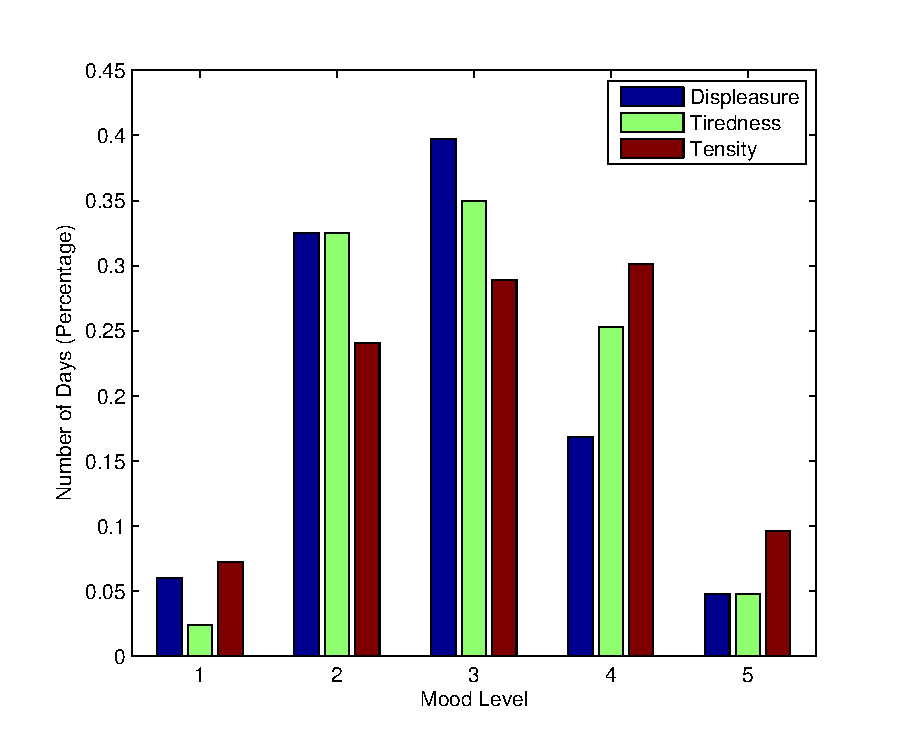
\includegraphics[width=15cm,height=10cm]{days}
  \caption{心境级别的分布}
  \label{mood:fig:mooddist}
\end{figure}

关于用户心境状态的时序分布方面,图\ref{mood:fig:moodcorr}展示了两个接连的时间槽(两天)内的心境状态差别分布。本图中,横轴表示这一时间槽与上一时间槽心境级别的差别(0代表没有差别)。从图中可以看出,每日的心境状态的时序关联关系非常显著,也即人们在连续的两天的心境状态通常是一致的,少有超过两个级别的非常极端的变化。这也验证了心境理论中的心境相对稳定性特征。
\begin{figure}[htbp]
  \centering
    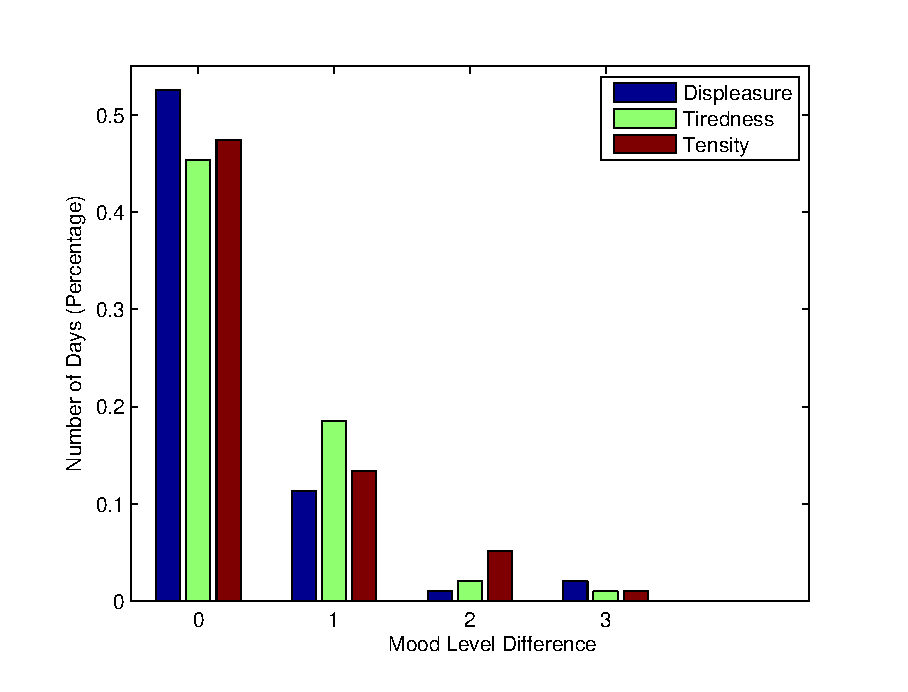
\includegraphics[width=15cm,height=10cm]{diff}
  \caption{连续两天内的心境差别分布}
  \label{mood:fig:moodcorr}
\end{figure}

在日常行为特征方面,我们分析了不同特征与心境状态之间的关联关系。作为示例,图\ref{mood:fig:minormotion}中展示了微动作与心境状态之间的关系。从图中可以看出,随着不愉快程度以及紧张程度的提高,微动作的数量也基本呈增加状态;而心境的活跃维度与微动作之间便没有显著的关联关系。从这可以看出,从传感器数据得到的日常行为特征与心境状态存在着关联关系,这也为使用贝叶斯方法利用手机感知的行为特征进行心境状态的评估提供了合理性。

\begin{figure}[htbp]
  \centering
    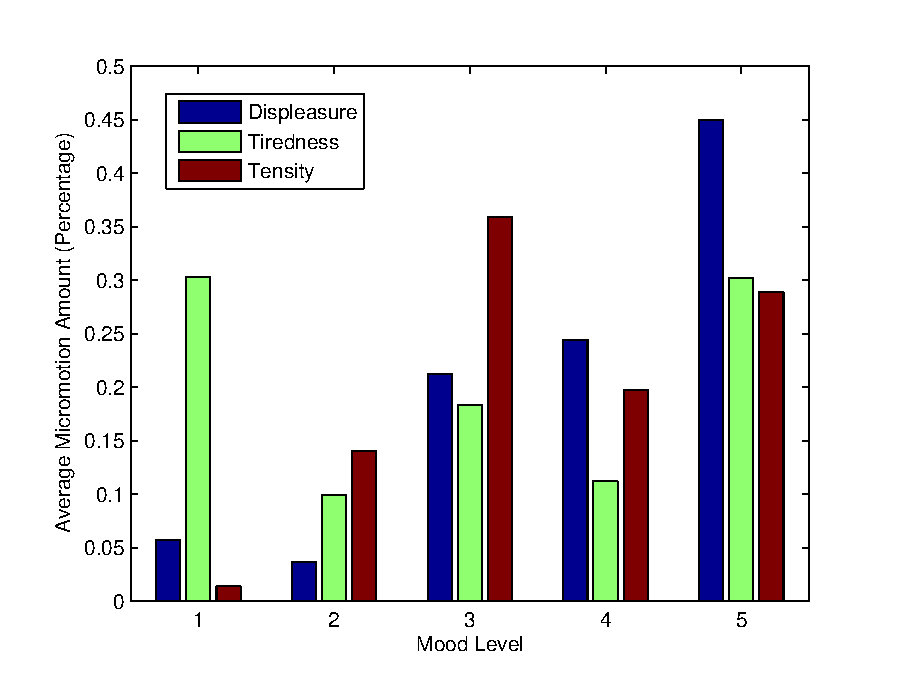
\includegraphics[width=15cm,height=10cm]{motion}
  \caption{不同心境状态下的微动作数量分布}
  \label{mood:fig:minormotion}
\end{figure}

\subsection{模型描述}
\label{mood:sec:ModelDescription}

基于对数据的观察结果,本文提出了一种基于因子图模型的分类算法,称为``社交-特征因子图''(Social-Featured Factor Graph,SFFG)。因子图模型是一个二元图模型,用以描述一类学习目标为包含多个变量的复杂全局函数的算法。这类算法中,全局目标函数被分解为多个``本地''函数的乘积,每个``本地函数''只包含全局函数的变量的一个较小的子集,并且函数形式更为简单\cite{factorgraph, followback}。

在详细描述模型之前,首先阐明几个基于实验数据观察的合理假设。首先,为简化模型,假设用户的心境状态具有马尔可夫性,也即用户上一时间槽内的心境状态只能影响紧接着的下一时间槽的心境状态,并通过对下一时间槽心境状态的影响来影响未来。这个性质可以如下表示:给定$m_i^{(t-1)}$,$m_i^{(t)}$与$m_i^{(t')}$对于所有$t' \leq t-2$条件独立。
我们也假设同一用户在同一时间槽内的不同行为特征关于此时间槽内的心境状态是条件独立的,也即给定$m_i^{(t)}$,所有$x_{ij}^{(t)} \in X_i^{(t)}$条件独立。 

基于上述的观察和假设,本文定义如下的因子函数:

\begin{itemize}
  \item \textbf{时序关联因子:} $tc(m_i^{(t-1)}, m_i^{(t)})$. 这个因子函数反映了心境的稳定性。基于前文提到的马尔可夫性假设,用户心境状态的衰减可以按如下函数建模:
  \begin{equation}
    tc(m_i^{(t)}, m_i^{(t-1)}) = exp\{-\lambda _i \| m_i^{(t)} -m_i^{(t-1)} \| \}
    \label{mood:tc}
  \end{equation}
  其中参数$\lambda_i$表示了用户\textit{i}的心境状态的时序衰减程度。  
  \item \textbf{特征关联因子:} $\textbf{c}(m_i^{(t)}, x_{ij}^{(t)})$. 每个用户行为特征$x_ij^{t}$都对用户$i$的心境$m_i^{(t)}$在不同维度上有不同程度的影响。本文使用朴素贝叶斯策略来建模特征的影响,用贝叶斯理论来建模$c(m_i^{(t)}, x_{ij}^{(t)})$,即先前观测到的取值组合具有更高的因子函数取值。

根据前文的假设,行为特征之间具有条件独立性,因此所有特征关联因子可以以如下的形式组合:
\begin{equation}
fe(m_i^{(t)}, \mathbf{x}_i^{(t)}) = \frac{1}{Z_\beta}exp\{\mathbf{\beta}^T\mathbf{c}(m_i^{(t)}) \mathbf{x}_i^{(t)}\}
\label{mood:fe}
\end{equation}
其中$\textbf{c}$代表特征关联因子向量,$\mathbf{\beta}$是一个权重向量,用来控制每个特征的相对权重,而$\frac{1}{Z_1}$为归一化因子。 

\item \textbf{社交关联因子:} $sc(m_i^{(t)}, m_j^{(t)})$. 社会关系的当前心境状态之间存在着相互影响。社交影响用如下函数建模:
\begin{equation}
sc(m_i^{(t)}, m_j^{(t)}) = exp\left\{ \alpha_i e_{ij}^{(t)} * (m_i^{(t)} -m_j^{(t)}) \right\}
\label{mood:sc}
\end{equation}
\end{itemize}
其中,$e_{ij}^{(t)}$为社交影响(参见定义\ref{mood:equ:e})。$\alpha_i$为权重参数,反应用户$i$的心境对于社会关系的易受影响程度。

最终,给定一个网络$G^{(t-1)} = \{\mathbf{V}, \textbf{E}^{(t-1)}, \mathbf{X}^{(t-1)}, \mathbf{m}^{(t-1)}\}$,以及当前的状态$\mathbf{X}^{(t)}$及$\mathbf{E}^{(t)}$,根据公式(\ref{mood:tc}),(\ref{mood:fe})与(\ref{mood:sc}),$M$上的联合概率分布为: 
\begin{equation}
\begin{split}
p(m|G^{(t-1)},& \mathbf{X}^{(t)}, \mathbf{E}^{(t)}) \\
=& \prod_i tc(m_i^{(t-1)}, m_i^{(t)})\,fe(m_i^{(t)}, \mathbf{x}_i^{(t)})\, sc(y_i^{t},H(y_i^{t-1})) \\
=& \frac{1}{Z} \prod_i exp \bigg\{-\lambda _1 \| m_i^{(t)} -m_i^{(t-1)} \|  \\
& + \mathbf{\beta}^T\mathbf{c}(m_i^{(t)}) \mathbf{x}_i^{(t)} + \sum_j \left(\alpha_i e_{ij}^{(t)} * (m_i^{(t)} -m_i^{(t-1)})\right) \bigg \}
\end{split}
\label{mood:target}
\end{equation}
其中$\mathbf{\lambda}$,$\mathbf{\beta}$及$\mathbf{\alpha}$为模型参数,$\frac{1}{Z}$为全局归一化因子。

SFFG的图形化表示见图\ref{mood:fig:sffg}。每个用户有其所有行为特征的取值以及心境状态,用户之间由社交影响因子$e$相连。输入的网络通过因子函数$tc$,$fe$以及$sc$生成全局概率分布

\begin{figure}[htbp]
  \centering
  \scalebox{0.75}{
    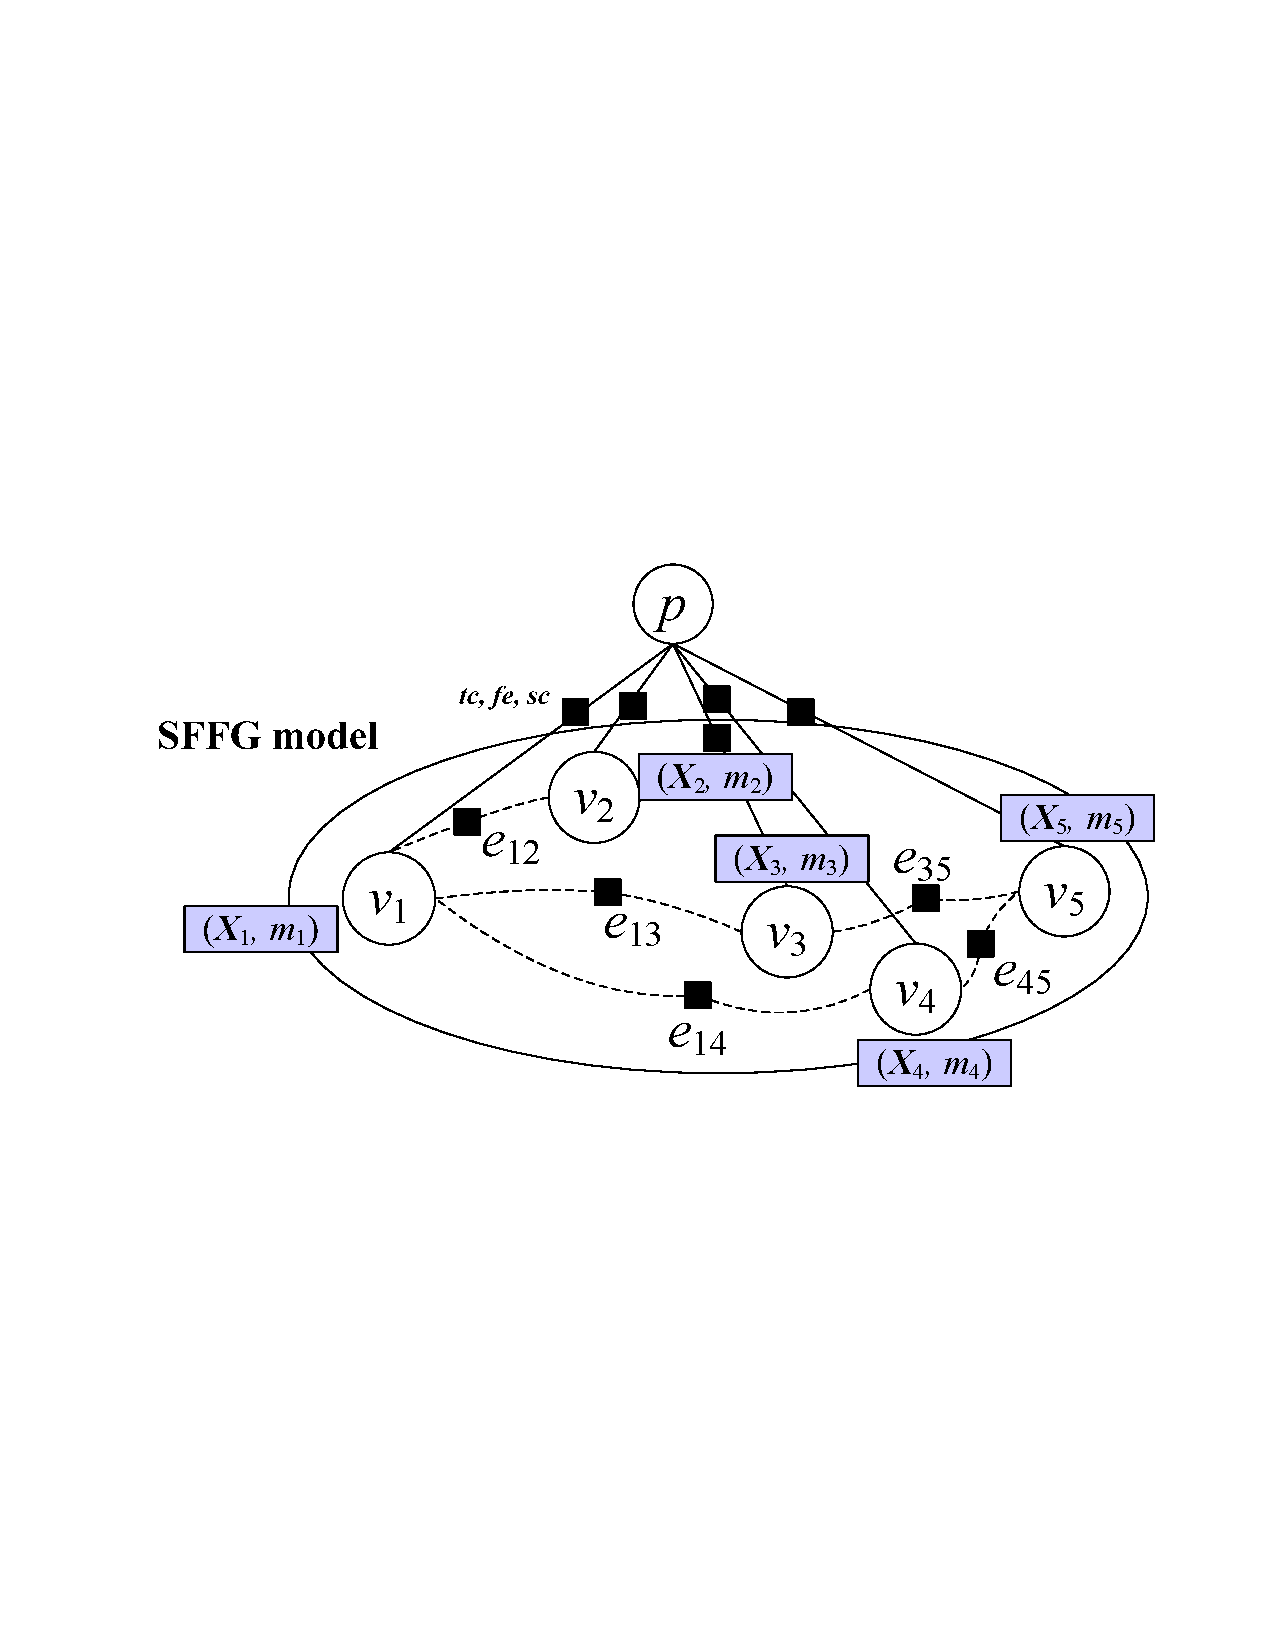
\includegraphics{sffg}
    }
  \caption{Visual depiction of SFFG model}
  \label{mood:fig:sffg}
\end{figure}


\subsection{SFFG模型学习}
\label{mood:sec:ModelLearning}
此模型的学习过程,也即训练参数$\theta = (\mathbf{\lambda}, \mathbf{\beta}, \mathbf{\alpha})$的最佳配置,以最大化给定训练数据上心境状态的对数似然:
\begin{equation}
\theta^* = {argmax}_\theta\left\{log\ p(\mathbf{m}|G^{(t-1)}, \mathbf{X}^{(t)}, \mathbf{E}^{(t)}, \theta)\right\}
\end{equation}
为了学习这样一个含有众多参数及全局归一化因子$Z$的目标函数,本文参与了基于Metropolis-Hastings (MH)抽样的算法。Metropolis-Hastings (MH)抽样算法为马尔可夫链蒙特卡洛方法(Markov-chain Monte Carlo,MCMC)的一个特例\cite{mh}\cite{socialEmotion}。

\begin{algorithm}
%\SetAlgoLined
\KwIn{learning rate $\eta$ which is the parameter that reflects the speed of learning}
\KwOut{optimal parameter $\theta = (\mathbf{\lambda}, \mathbf{\beta}, \mathbf{\alpha})$}

Initialize $\theta$;

\Repeat{Convergence}{
\% sample a new target variable configuration $\mathbf{m'}$
\[\mathbf{m'} \leftarrow q(\mathbf{m});\]
\[\tau \sim min(\frac{p(\mathbf{m'}|G^{(t-1)}, \mathbf{X}^{(t)}, \mathbf{E}^{(t)}, \theta)}{p(m|G^{(t-1)}, \mathbf{X}^{(t)}, \mathbf{E}^{(t)}, \theta)}, 1);
\]
%
\% generate a 0-1 random variable  $s$
\[s \sim Bernoulli(\tau, 1 - \tau);\]
%

\If{(s = 1)} 
{\
\% accept the new configuration $\mathbf{m'}$
\[ \mathbf{m} \leftarrow \mathbf{m'}; \]
\uIf{$(Err(\mathbf{m'}) < Err(\mathbf{m}) \Delta Ex|_\theta < 0) $}
{\[ \theta^{new} \leftarrow \theta^{old} + \eta(\Delta Ex|_\theta); \]}
\ElseIf{$(Err(\mathbf{m'}) > Err(\mathbf{m})  \Delta Ex|_\theta \geq 0) $}
{\[ \theta^{new} \leftarrow \theta^{old} - \eta(\Delta Ex|_\theta); \]}

}
}

\caption{模型学习算法}
\label{mood:alg:learning}
\end{algorithm}

MH算法分两个步骤。在第一步中,采用一个简单的抽样方法$q(\mathbf{m})$,从原目标配置$\mathbf{m}$中生成候选的新目标配置$\mathbf{m'}$。$q(\mathbf{m})$为简单地在目标配置空间全集$M$上按$m$的分布随机抽样。在第二步中,新的目标配置以概率$\tau$被接受:
\begin{equation}
\tau \sim min(\frac{p(\mathbf{m'}|G^{(t-1)}, \mathbf{X}^{(t)}, \mathbf{E}^{(t)}, \theta)}{p(m|G^{(t-1)}, \mathbf{X}^{(t)}, \mathbf{E}^{(t)}, \theta)}, 1)
\end{equation}

而后,如果新的配置$\mathbf{m'}$被接受,则更新模型参数$\theta$。参数的更新过程去觉得新旧配置$\mathbf{m}$与$\mathbf{m'}$的错误率$Err$,以及两个配置的对数似然差别$\Delta Ex|_\theta$: 
\[\Delta Ex|_\theta = Ex|_\theta (\mathbf{m'}) - Ex|_\theta(\mathbf{m})\] 
其中$Ex(\mathbf{m})$为公式\ref{mood:target}的指数部分($exp\{...\}$中包含的部分)

\section{算法评估}\label{mood:evaluation}


实验获取的数据集包含了2,872,311条手机传感器数据(包括加速度传感器,地理位置等),3,169条短信息记录,以及5,871条通话记录。 

收集到的原始数据按上文描述被聚合成特征,每个被试的每个特征每天有一个取值。
自报告的心境数据同样被聚合成每天一个取值(包含三个维度)。对于每天标注了多次心境状态的用户,取其所有标注值的加权平均值作为当天的心境状态,其中越晚的标注值权值越高。
被试用户被要求在每天的活动时间内在其手机上运行应用,并在夜间将要休息之前停止手机应用的数据采集,因为睡眠期间的传感数据并不能有效反应日常的行为,因此不能用来做每日心境评估。

由于此学习问题为针对离散的顺序级别的分类问题,本文采用准确度(预测的心境状态级别与报告的数据完全一致的人·天数占所有人·天数的比例),以及均方根误差(RMSE,root-mean-square error)作为模型表现的度量。模型的训练和测试采用了5份交叉验证的方法。

准确度的定义为: 
\[ accuracy = \frac{\sum_{u,d}{I_{(x_u^{(d)} = \widetilde{x}_u^{(d)})}}}{UD}
\]
均方跟误差的计算方法为:
\[
RMSE = \sqrt{\frac{\sum_{u,d}{{(x_u^{(d)} - \widetilde{x}_u^{(d)})}^2}}{UD}}
\]
其中$x_u^{(d)}$为评估结果,$\widetilde{x}_u^{(d)}$为实际的用户自报告值。$x$可以使三个心境维度$d$,$ti$或$te$中的任意一个。$I_s$ 为示性函数:当$s$为真时$I_s = 1$,反之$I_s = 0$。$U$和$D$为测试集中总的\textit{人·天}数。 


\begin{table}[htbp]
  \centering
  \caption{使用部分SFFG下MoodMiner的评估表现}
  \label{mood:tab:Performance}
    \begin{tabular}{|l|c|r|}
      \hline
      目标 & 准确度 & 均方根误差 \\
      \hline
      愉快度 & 52.58\% & 1.446 \\
      兴奋度 & 45.36\% & 1.519 \\
      放松度 & 47.42\% & 1.564 \\
      \hline
    \end{tabular}
\end{table}

\begin{table}[htbp]
  \centering
  \caption{使用完整SFFG下MoodMiner的评估表现}
  \label{mood:tab:Performance2}
    \begin{tabular}{|l|c|r|}
      \hline
      目标 & 准确度 & 均方根误差 \\
      \hline
      愉快度 & 71.68\% & 0.34 \\
      兴奋度 & 65.15\% & 0.361 \\
      放松度 & 65.60\% & 0.433 \\
      \hline
    \end{tabular}
\end{table}
使用SFFG评估模型,本文进行了两组模型实验。第一组实验中,只考虑了有时序因子及简单行为特征因子(包括地理位置,加速度,短信息频率,通话频率以及声音强度),模型的总体准确度稍低于50\%;第二组实验中,采用了完整的SFFG模型,包含了复杂的行为特征因子(活动姿态以及微动作),并且添加了社交影响因子。第二组实验的准确度提高了约20个百分点,达到了70\%左右。

\textbf{讨论.} 
评估模型的表现比较令人满意,最终达到了70\%左右的精度。最终输出的误差来源于多个方面。首先,由于心境天然的主观性,手机传感数据,通讯数据以及历史心境数据均有可能在一定情况下无法反映心境的波动 - 用户心境可能无任何征兆地突然变化。其次,人们在日常使用手机的模式上也存在很大的不同,使得统一的模型在不同用户身上可能出现较大的表现差别,很难让模型对于所有用户均有良好的表现。对于某些用户,功能强大的智能手机只有来接打电话和发信息,其余时间并不接触,使得本评估方法失败。另外,有些可能对心境评估产生作用的手机数据并未被采集,例如特定类型手机应用的使用情况;以及手机短信、电话功能外由应用提供的通讯方式(如\textit{Talkbox}\footnote{\url{http://talkboxapp.com/en/home}}及\textit{Skype}\footnote{\url{https://play.google.com/store/apps/details?id=com.skype.raider}}等)的使用情况
这些缺失的数据同样会影响模型最终的表现。


\section{本章小结}\label{mood:conclusion}

本章提出了一个单纯利用智能手机数据,通过用户行为分析来评估个人日常心境状态的新颖方法。首先定义了从手机数据中解析出的若干行为特征,而后提出了一个基于因子图模型的结合行为特征,时序关联和社交关联的心境评估方法。相较于传统的方法,这一方法具有用户干预少,客观,方便等优点,15个被试者延续了30天的实验表明,这一方法达到了令人满意的模型表现。
 

% % use section* for acknowledgement
% \section*{Acknowledgment}

% This work was supported in part by the National Science Foundation (NSF) of China, with grant No.61170212.

% % references section



% 如果要把编号的两个图形并排,那么小页就非常有用了:
% \begin{figure}
% \begin{minipage}{0.48\textwidth}
%   \centering
%   
\includegraphics[height=2cm]{thu-whole-logo}
%   \caption{并排第一个图}
%   \label{mood:fig:parallel1}
% \end{minipage}\hfill
% \begin{minipage}{0.48\textwidth}
%   \centering
%   
\includegraphics[height=2cm]{thu-whole-logo}
%   \caption{并排第二个图}
%   \label{mood:fig:parallel2}
% \end{minipage}
% \end{figure}

% 李氏子蟠,年十七,好古文、六艺,经传皆通习之,不拘於时,学於余。余嘉其能行古
% 道,作师说以贻之。

% \hfill \pozhehao 韩愈(唐)

